\documentclass[11pt, oneside]{article}   	% use "amsart" instead of "article" for AMSLaTeX format
\usepackage{geometry}                		% See geometry.pdf to learn the layout options. There are lots.
\geometry{letterpaper}                   	% ... or a4paper or a5paper or ... 
%\geometry{landscape}                		% Activate for rotated page geometry
\usepackage[parfill]{parskip}    	% Activate to begin paragraphs with an empty line rather than an indent
\usepackage{graphicx}				% Use pdf, png, jpg, or eps§ with pdflatex; use eps in DVI mode
								% TeX will automatically convert eps --> pdf in pdflatex		
\usepackage{amssymb}
\usepackage{amsmath}
\usepackage{hyperref}
\usepackage{makecell} % Add this to your preamble



\title{scPerturb: single cell perturbation}
\author{Sicheng Yi}
\date{05/02/2025}		

\begin{document}
\maketitle
\begin{abstract}
This project aims to understand how drug compounds alter single cell gene expression levels and whether the up- or down-regulation effects will suppress cancer cell lines among PBMC peripheral white blood cells. Using deep learning models such as MLP and Transformers, we can improve the prediction on how the drugs change the differential expression level of T, B, NK, and myeloid cells to find a potential drug candidate to cure blood cancer leukemia. 
\end{abstract}


\section*{Introduction}

Each year millions of people die of cancer and acute leukemia is very prevalent. Researchers want to understand how the different chemical drug compounds affect gene regulation in peripheral white blood molecular cells (PBMC). The setup of the experiment is shown in Figure~\ref{fig:pbmc}. 

\begin{figure}[htbp]
  \centering
  \includegraphics[width=0.8\textwidth]{pbmc.png}
  \caption{Visualization of PBMC data.}
  \label{fig:pbmc}
\end{figure}

Blood samples from both healthy and cancer patients are collected and analyzed via single cell RNA and ATAC chromatin peak sequencing analysis. More than 140,000 individual cells are collected and perturbed by 144 chemical compounds to observe the change in expression levels of 18,000+ genes. Those cells are bulked and grouped into several categories: T cells CD4+, T cells CD8+, NK cells, B cells, Myeloid cells. 

As part of the 2023 NeurIPS Kaggle competition, researchers want the ML community to develop tools and models to predict the differential expression levels of each genes based on the various cell types and small molecular compounds. 

One of the challenges of this problem is that the input dimension of cell type and drug compound is a lot smaller than the output dimension for the gene expression level for over 18000 genes. Another challenge of this problem is that training data is mostly focused on T and NK cells, while the test data is concentrated in the B cells and Myeloid cells. 

This project aims to augment the input features and deploy deep learning models such as MLP and transformers to better learn and generalize to the unseen test dataset. 


\section*{Related Work}

1. RandomSmiles  \cite{RandomSmiles} 

This study discusses how different atom orderings can lead to varied SMILES strings and how RDKit addresses this with built-in fixes. SMILES is the 1D molecular representation of the drug compounds. The authors introduced this 1D string representation and the biological property such as bond strength and molecular binding sites that will play critical roles in the gene regulation. 


2. scPerturb \cite{scPerturb}

This resource compiles 44 publicly available single-cell perturbation-response datasets, including transcriptomics and proteomics data. It introduces energy statistics (E-statistics) for quantifying perturbation effects and significance testing, facilitating comparison and integration across datasets.

3. scRNA-PBMC \cite{scRNA-PBMC}

This study performed single-cell RNA sequencing on 1.3 million PBMCs white blood cells from 120 individuals exposed to different pathogens, providing insights into gene expression and regulatory responses influenced by genetic background and pathogen exposure.




\section*{Datasets}

As part of the scPerturb NeurIPS 2023 Kaggle Competition, the researcher collected healthy and cancer patient's PBMC white blood cells and used 144 drug compounds to perturb the 18000+ genes to get their differential expression levels. More than 140,000 individual cells are bulked into several cell types: T cells CD4+, T cells CD8+, NK cells, B cells, Myeloid cells. 

The main dataset is held in de-train parquet file. The rows of this data are the cell type + small chemical compound pairs. Most of the columns are the 18,000+ individual genes and each entries are the numerical differential expression levels that the model needs to learn. There are also SMILES column which shows the 1D string representation of the actual chemical compound of the 144 drugs. Training data mostly contains the T cells, NK cells, and a few B cells and Myeloid cells. The unseen test data contains mostly just the B cells and Myeloid cells. 


\begin{table}[htbp]
\centering
\small
\begin{tabular}{|l|l|l|l|c|r|r|}
\hline
\textbf{cell\_type} & \textbf{sm\_name} & \textbf{sm\_lincs\_id} & \textbf{SMILES} & \textbf{control} & \textbf{A1BG} \\
\hline
NK cells & Clotrimazole & LSM-5341 & \makecell[l]{Clc1ccccc1C(c1ccccc1)\\(c1ccccc1)n1ccnc1} & False & 0.104720  \\
\hline
T cells CD4+ & Clotrimazole & LSM-5341 & \makecell[l]{Clc1ccccc1C(c1ccccc1)\\(c1ccccc1)n1ccnc1} & False & 0.915953 \\
\hline
T cells CD8+ & Clotrimazole & LSM-5341 & \makecell[l]{Clc1ccccc1C(c1ccccc1)\\(c1ccccc1)n1ccnc1} & False & -0.387721  \\
\hline
T regulatory cells & Clotrimazole & LSM-5341 & \makecell[l]{Clc1ccccc1C(c1ccccc1)\\(c1ccccc1)n1ccnc1} & False & 0.232893  \\
\hline
\end{tabular}
\caption{differential expression level of each genes perturbed by drug among cell types}
\label{tab:de_train}
\end{table}

The main training data is shown in Table~\ref{tab:de_train}. The numerical values of the differential expression level of each genes shows how significant each drug will boost or suppress  gene expression. A positive number (+) means up-regulation, and a negative  number (-) means down regulation. Larger the absolute value, the large statistical significance the perturbation effect will be. 

The entry of the SMILES column is the 1D string representation of the 144 drug compounds. Figure~\ref{fig:smiles} shows the 3D structure of the 1st small molecule clotrimazole. 


\begin{figure}[htbp]
  \centering
  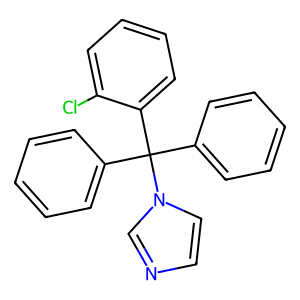
\includegraphics[width=0.3\textwidth]{smiles1.png}
  \caption{Visualization of clotrimazole.}
  \label{fig:smiles}
\end{figure}

\begin{figure}[htbp]
  \centering
  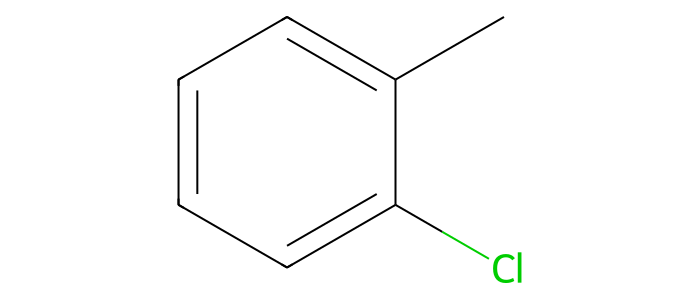
\includegraphics[width=0.3\textwidth]{smiles1-split1.png}
  \caption{clotrimazole sub module 1}
  \label{fig:smiles1}
\end{figure}

\begin{figure}[htbp]
  \centering
  
\includegraphics[width=0.3\textwidth]{smiles1-split2.png}
  \caption{clotrimazole sub module 2}
  \label{fig:smiles2}
\end{figure}

Figure~\ref{fig:traintest} shows that the Train and Test data also has unbalanced distribution. Train data is concentrated mostly on various types of the T cells and NK cells. The unavailable test data mostly focuses on the B cells and Myeloid cells. 

\begin{figure}[htbp]
  \centering
  
\includegraphics[width=1.0 \textwidth, height=0.3 \textwidth ]{train-test-split.png}
  \caption{Split of Training Test data}
  \label{fig:traintest}
\end{figure}


\section*{Approach and Methodology}

\subsection{EDA}

First step I took is to run exploratory data analysis to identify on which genes are more important than the others. Gene CD69 is one of the common blood cancer cell lines that is over expressed among the healthy patients shown in Figure~\ref{fig:CD69healthy}, compare to the cancer patients shown in Figure~\ref{fig:CD69MPAL}. 

For the cancer patients, the gene CD69 is over expressed among the T/NK cells, as well as in the Myeloid cells. It shows that the over expression of gene CD69 will have a strong correlation of blood cancer. There are also over 18000 genes analyzed, so any drug that can down regulate such cancer prone gene will be an ideal candidate for the cure to blood cancer. 

\begin{figure}[htbp]
  \centering
  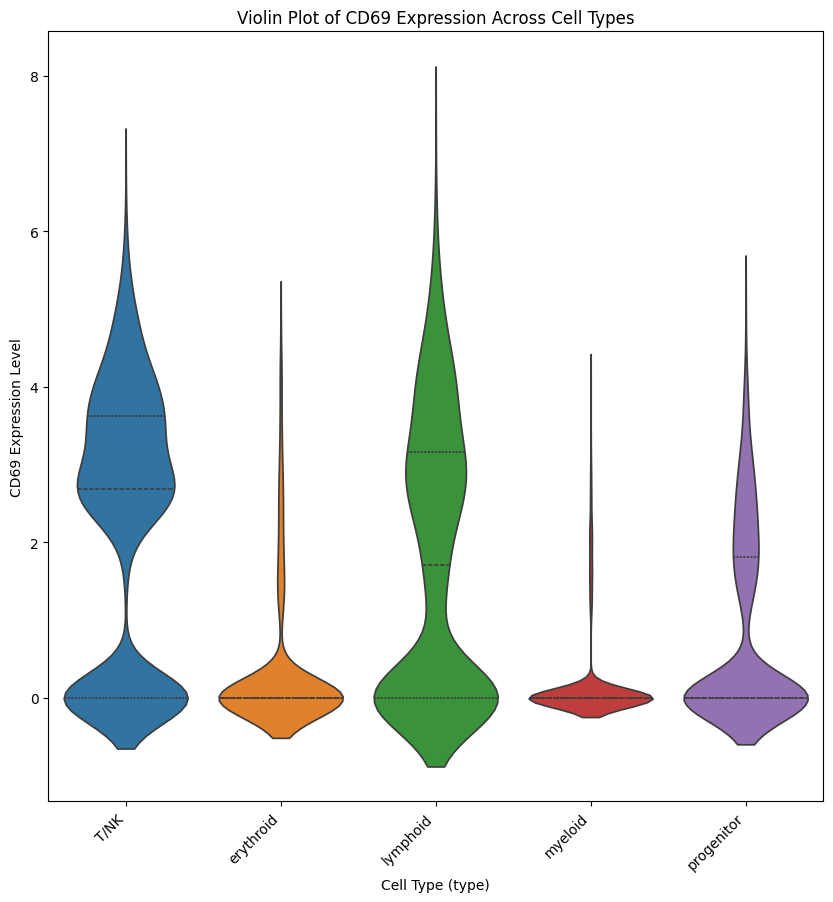
\includegraphics[width=0.3\textwidth]{CD69-health.png}
  \caption{gene CD69 healthy}
  \label{fig:CD69healthy}
\end{figure}


\begin{figure}[htbp]
  \centering
  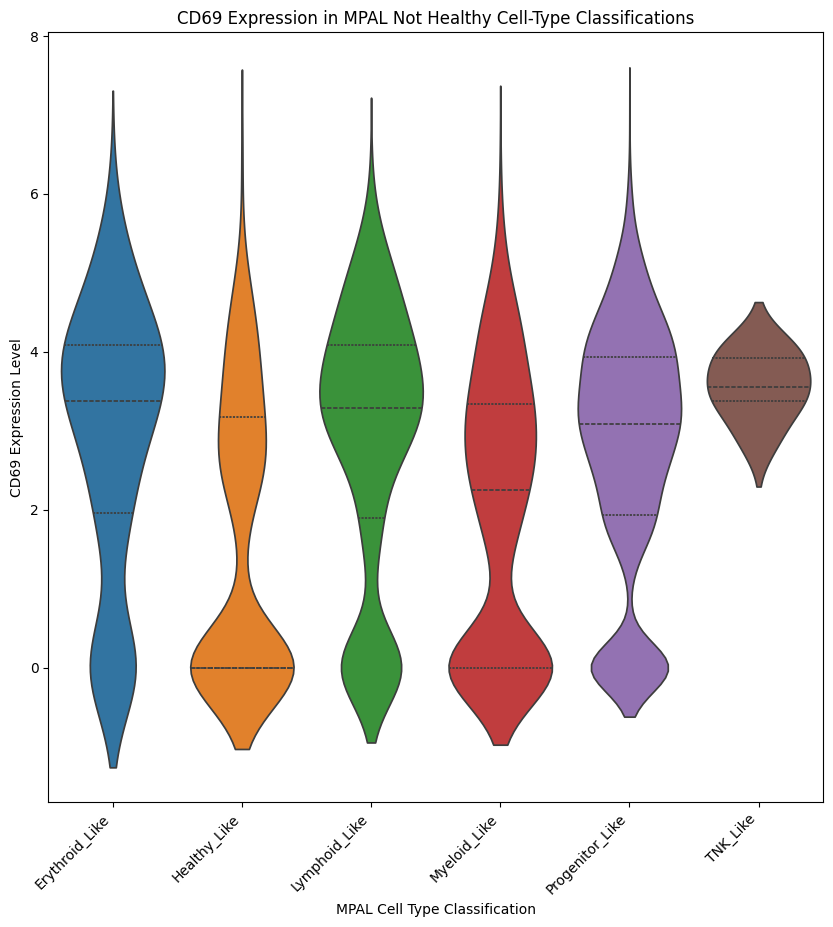
\includegraphics[width=0.3\textwidth]{CD69-MPAL.png}
  \caption{gene CD69 MPAL leukemia}
  \label{fig:CD69MPAL}
\end{figure}


\subsection{Data Augmentation}

A challenge of this project is that the input features only include several categorical columns, namely the cell types, the sm drug compounds, SMILES strings, and controls, yet the model needs to output numerical gene expression levels for over 18,000+ genes (columns) across all the cell types drug pairs. It's important to augment the input features prior to the ML models. 

First, for both the training and test data, I add the numerical features such as mean, standard deviation, and median of the gene differential expression levels for both the sm drug and cell types as the input features. This dramatically improves model performance as the baseline statistics served as a general baseline for the model. 

Second, I generate more features based on the SMILES string. For example, Figure~\ref{fig:smiles} shows the full small drug compound clotrimazole. I will break down the molecule into many sub units such as in Figure~\ref{fig:smiles1} and Figure~\ref{fig:smiles2}. I will then make a sparse count matrix to count the occurrence of each sub units from the 144 drugs. And this coount matrix will serve as part of the input features. 

Third, to future augment the data, I also use the RDKIT Chem package to get the Morgan Fingerprint features from the SMILE drug compounds. The fingerprint is a numerical features to denote the strength and the location of the chemical bonds of the molecules. By augmenting the SMILES features, the model is able to learn more biological properties during the regression. Without the additional features, the model can only learn the name and the 1D string representation of the drug compounds.

Last but not the least, the cell type and drug compound columns are categorical, in order for the models to run, I need to preprocess the categorical features into numerical features by using one-hot encoder and label encoder. 


\subsection{Models}

\begin{figure}[htbp]
  \centering
  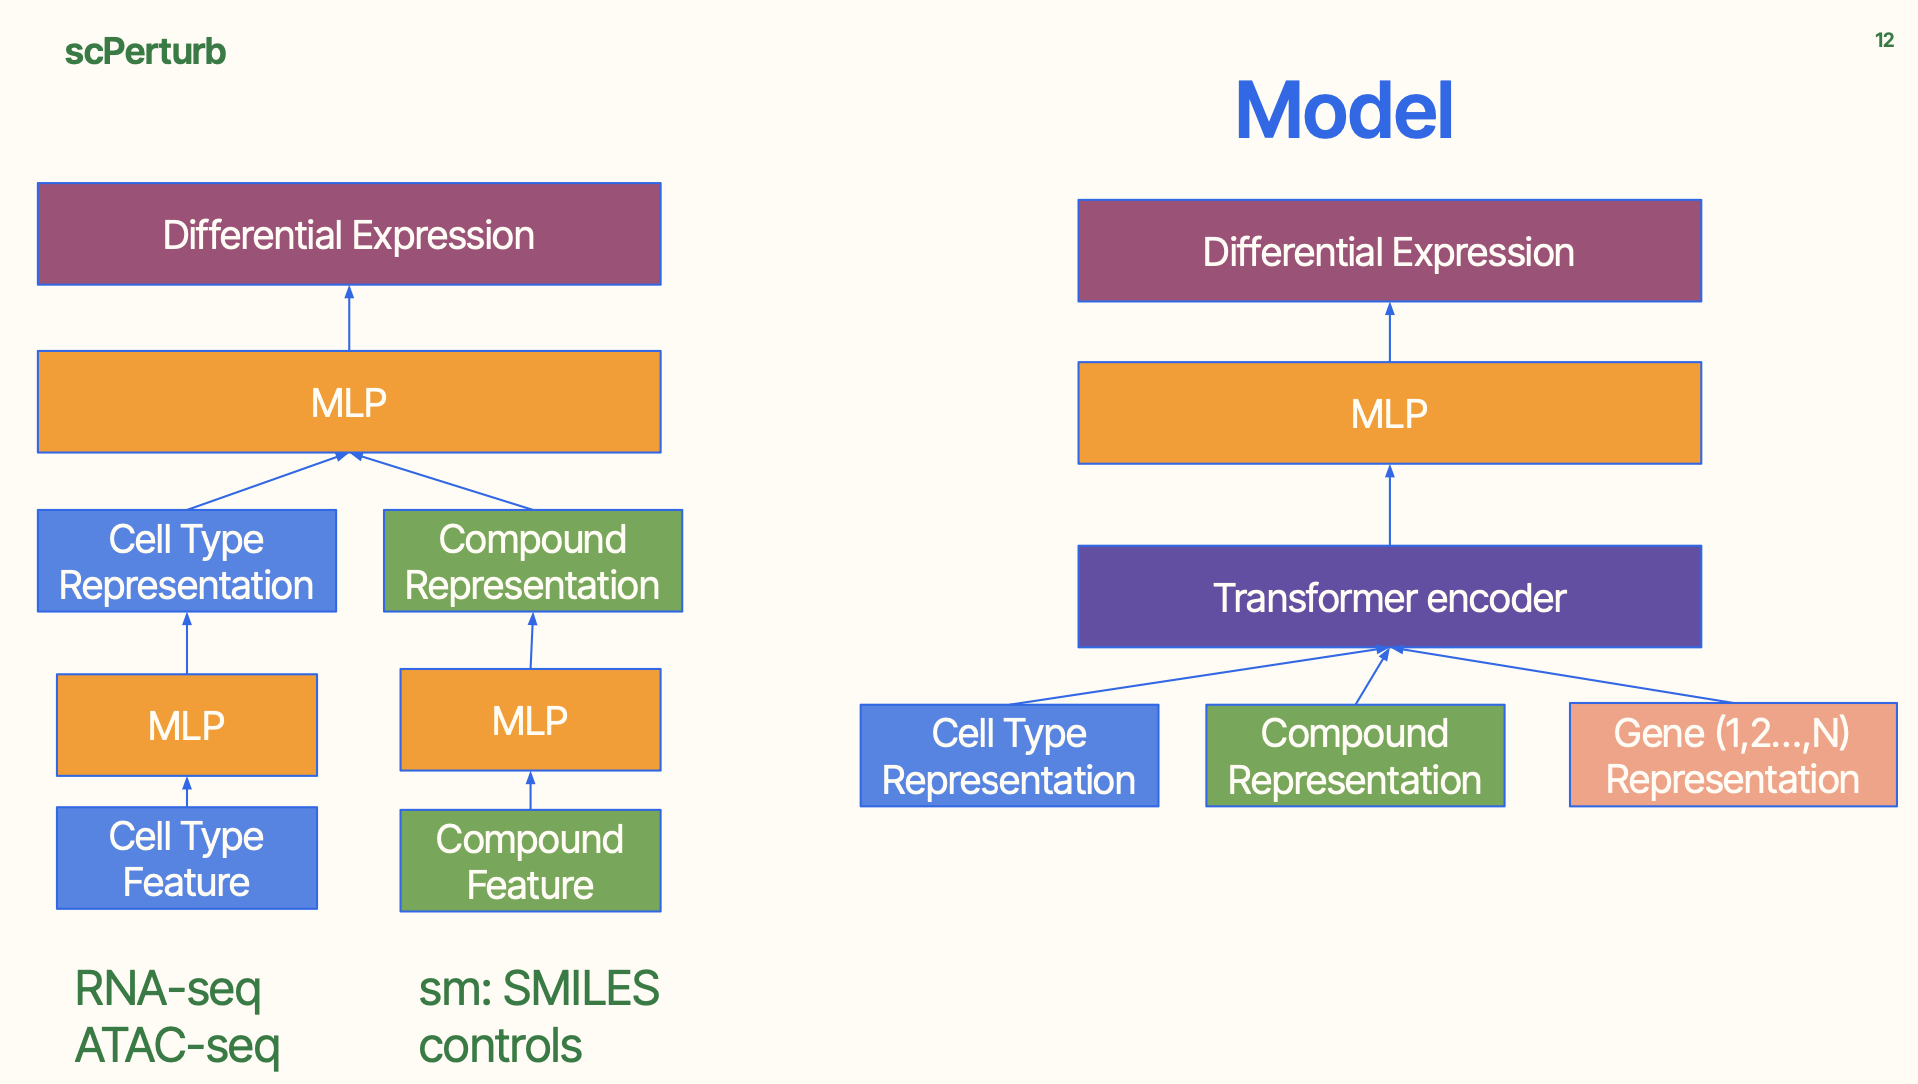
\includegraphics[width=1.0 \textwidth]{models.png}
  \caption{Models}
  \label{fig:models}
\end{figure}

Figure~\ref{fig:models} shows the 2 model architectures that I used. On the left I have the MLP model. On the right I have the Transformer model. 

For MLP, I use 2 separate MLP with 2 layers made of linear, batch norm, relu, dropout, etc., to get the cell type features and the drug compound features into the features space. The cell type features include the mean, std, median of the differential expression numerical values for the cell types and drug compounds. The SMILES features will include both the spare sub module count matrix as well as the Morgan Fingerprints. Then I concatenate both cell and drug features and then feed into another MLP in order to get out the differential expression for all cell-drug pairs and 18,000+ genes. 

For Transformer, I use 1 transformer encoder layer of 8 heads. I carefully separate out the categorical features and the numerical features. For categorical features like the cell type and drug compounds, I first make it Embedding so the model knows the values are categorical instead of numerical. I will then pass the categorical features into the transformer encoder layer. I will then concatenate the categorical features with the numerical features such as mean, std, median. Eventually I will pass everything into a MLP with 2 fully connected layers in order to get out the differential expression levels. 



\section*{Evaluation}

\begin{figure}[htbp]
  \centering
  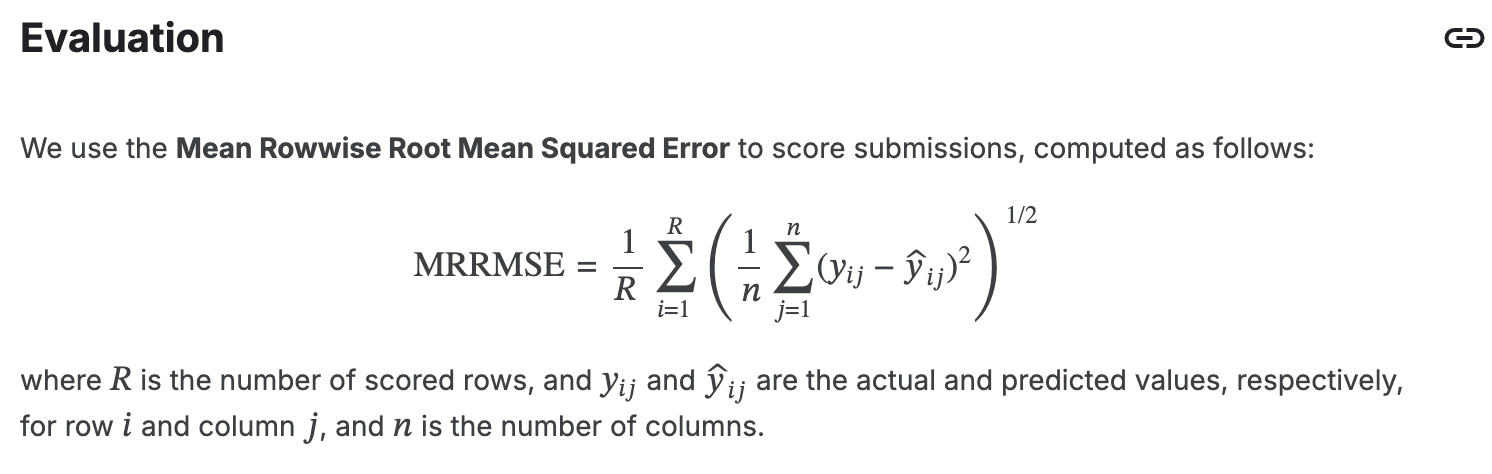
\includegraphics[width=1.0 \textwidth]{loss.png}
  \caption{MRRMSE loss}
  \label{fig:rmse}
\end{figure}

Figure~\ref{fig:rmse} shows the main evaluation metrics of our models. For each row of cell type - drug pairs, I first calculate the Root Mean Square Error between the actual y expression level and the predicted y hat expression level, and average across the n columns. Then for the R rows, I will average out all the RMSE to get out a single number. This metrics make sense because this problem is essentially a multi regression problem. 





\section*{Result}

\begin{figure}[htbp]
  \centering
  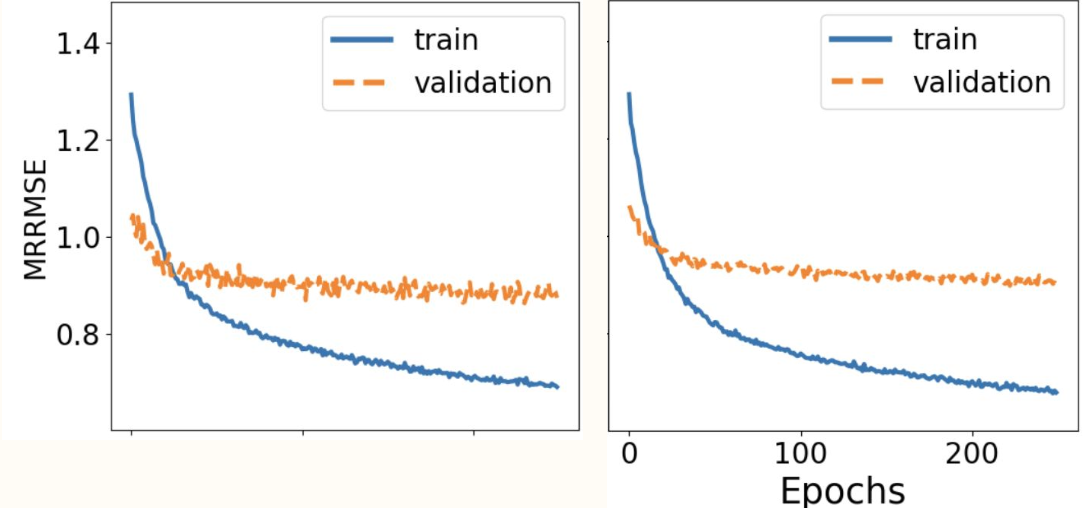
\includegraphics[width=1.0 \textwidth]{training.png}
  \caption{MRRMSE loss}
  \label{fig:training}
\end{figure}

Figure~\ref{fig:training} shows the trainging loss for both the MLP on the left and Transformers on the right. The MLP is slightly faster at loss convergence on the validation set, while Transformer needs to take slightly more epochs to achieve similar MRRMSE loss on the validation set. The graph also shows that the models might start to overfit on the training data because the validation loss tails off after roughly 100 epochs while the training loss decreases steadily. 

\begin{table}[htbp]
\centering
\begin{tabular}{|l|c|c|}
\hline
\textbf{MRRMSE} & \textbf{MLP} & \textbf{Transformer} \\
\hline
Validation & 0.86 & 0.90 \\
\hline
Test       & 0.93 & 0.87 \\
\hline
\end{tabular}
\caption{MRRMSE scores for MLP and Transformer models on validation and test sets.}
\label{tab:mrrmse_results}
\end{table}

Table~\ref{tab:mrrmse_results} shows the MRRMSE loss for the validation set and also the hidden test set on kaggle. MLP despite having better validation loss due to faster convergence compare to Transformer has higher loss on the actual test set. This means that the Transformer generalize to the unseen test set much better than the MLP. 

Transformer is able to capture longer term dependency between the features. Due to the huge unbalance of the cell type categories between the training and test data, Transformer appears to be more robust. 

For the best models on Kaggle, they all used an ensemble of 4-5 different models to achieve MRRMSE loss of roughly 0.75. 



\section*{Conclusion}

In conclusion, this project demonstrates that data augmentation and deep learning can significantly improve the prediction of gene expression changes in single cells exposed to chemical perturbations. By augmenting limited categorical inputs with statistical summaries, SMILES substructure counts, and molecular fingerprints, we enriched the feature space and enabled models to learn more meaningful biological patterns. Among the models tested, the Transformer model outperformed MLP on the unseen test data, highlighting its superior generalization in imbalanced settings where training and test cell types differ. While MLP offers faster convergence, Transformers are better suited for capturing complex relationships across high-dimensional gene expression outputs. Future work may include model ensembling, graph-based molecular encoders, and semi-supervised learning to further improve prediction accuracy and identify promising drug candidates for leukemia treatment.




\section*{Code}

The code for scPerturb is available on Github: 
\href{https://github.com/tigeryi1998/scPerturb}{Link}





\begin{thebibliography}{9}

\bibitem{RandomSmiles}
Arús-Pous, J., Johansson, S.V., Prykhodko, O. et al.
\textit{Randomized SMILES strings improve the quality of molecular generative models. J Cheminform 11, 71 (2019)}. https://doi.org/10.1186/s13321-019-0393-0


\bibitem{scPerturb}
Peidli S et al.
\textit{scPerturb: harmonized single-cell perturbation data. Nature Methods. (2024)}.
https://doi.org/10.1038/s41592-023-02144-y


\bibitem{scRNA-PBMC}
Oelen, R., de Vries, D.H., Brugge, H. et al.
\textit{Single-cell RNA-sequencing of peripheral blood mononuclear cells. Nature Communication 13, 3267 (2022)}.
https://doi.org/10.1038/s41467-022-30893-5





\end{thebibliography}

\end{document} 